%-------------------------------------------------------------------------------
%-------------------------------------------------------------------------------
\begin{frame}\begin{center}
	\LARGE\textbf{Introduction}
\end{center}\end{frame}
%-------------------------------------------------------------------------------
%-------------------------------------------------------------------------------
\begin{frame}
\begin{figure}\caption{Motivation}\centering
    \subfloat[Carneiro \& al. (2011)]{{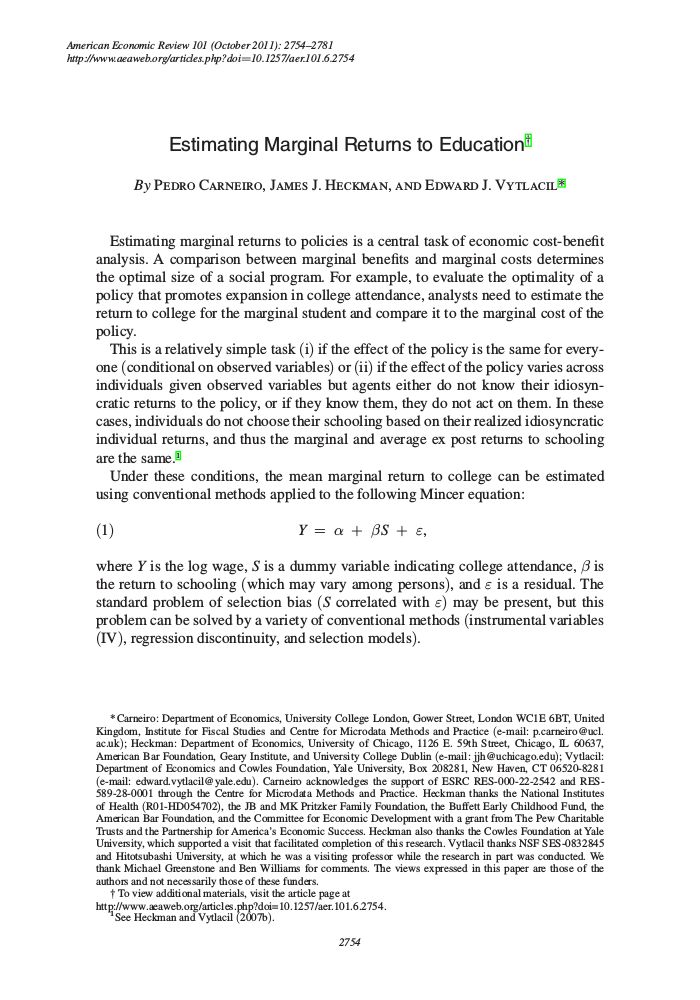
\includegraphics[width=4cm]{fig-cover-carneiro-2011.png}}}
    \qquad
    \subfloat[Carneiro \& al. (2003)]{{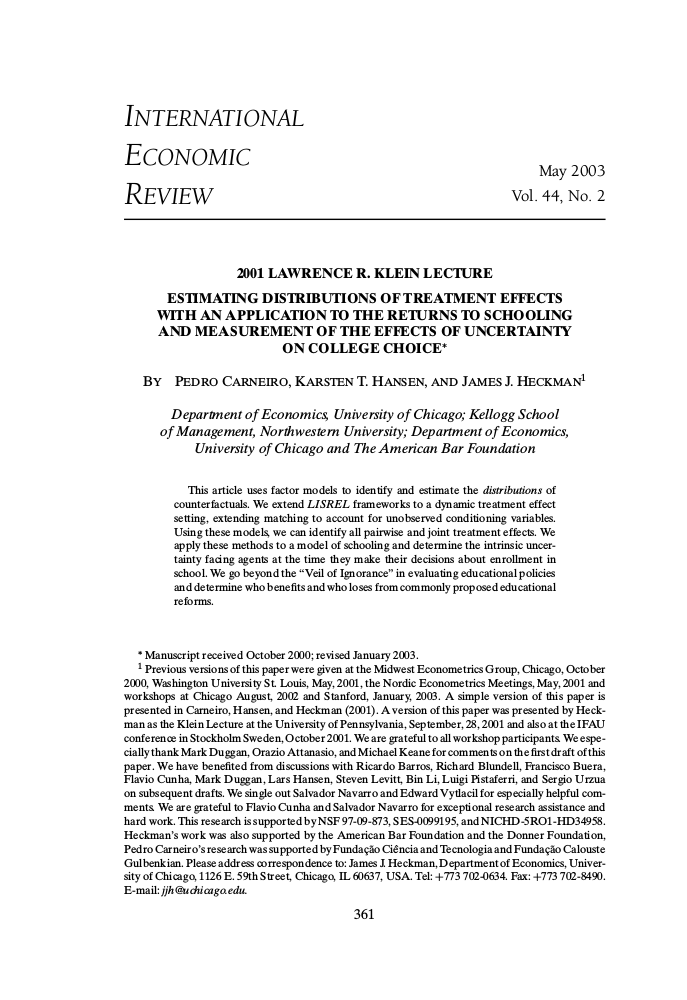
\includegraphics[width=4cm]{fig-cover-carneiro-2003.png}}}
\end{figure}
\end{frame}
%-------------------------------------------------------------------------------
%-------------------------------------------------------------------------------
\begin{frame}
	\textbf{\citeA{Heckman.2008} defines three policy evaluation tasks:}
	\begin{itemize}\setlength\itemsep{1em}
		\item Evaluating the impact of historical interventions on outcomes including their impact in terms of well-being of the treated and the society at large.
		\item Forecasting the impact of historical interventions implemented in one environment in other environments, including their impact in terms of well-being.
		\item Forecasting the impacts of interventions never historically experienced to various environments, including their impact on well-being.
	\end{itemize}
\end{frame}
%-------------------------------------------------------------------------------
%-------------------------------------------------------------------------------
\begin{frame}
	\textbf{Econometrics of policy evaluation}\\\vspace{0.3cm}
	\begin{itemize}\setlength\itemsep{1em}
		\item is important
		\item is complicated
		\item is multifaceted
	\end{itemize}
\end{frame}
%-------------------------------------------------------------------------------
%-------------------------------------------------------------------------------
\begin{frame}
\textbf{Numerous applications}\\\vspace{0.3cm}

	\begin{itemize}\setlength\itemsep{1em}
		\item labor economics
		\item development economics
		\item industrial economics
		\item health economics
	\end{itemize}
\end{frame}
%-------------------------------------------------------------------------------
%-------------------------------------------------------------------------------
\begin{frame}
\textbf{Numerous effects}\\\vspace{0.3cm}
	\begin{itemize}\setlength\itemsep{1em}
		\item conventional average effects
		\item policy-relevant average effects
		\item marginal effects
		\item distributional effects
		\item effects on distributions
	\end{itemize}
\end{frame}
%-------------------------------------------------------------------------------
%-------------------------------------------------------------------------------
\begin{frame}
\textbf{Numerous estimation strategies}\\\vspace{0.3cm}
	\begin{itemize}\setlength\itemsep{1em}
		\item instrumental variables
		\item (quasi-)experimental methods
		\item matching
	\end{itemize}
\end{frame}
%-------------------------------------------------------------------------------
%-------------------------------------------------------------------------------
